% Created by tikzDevice version 0.12.3.1 on 2021-03-17 17:12:35
% !TEX encoding = UTF-8 Unicode
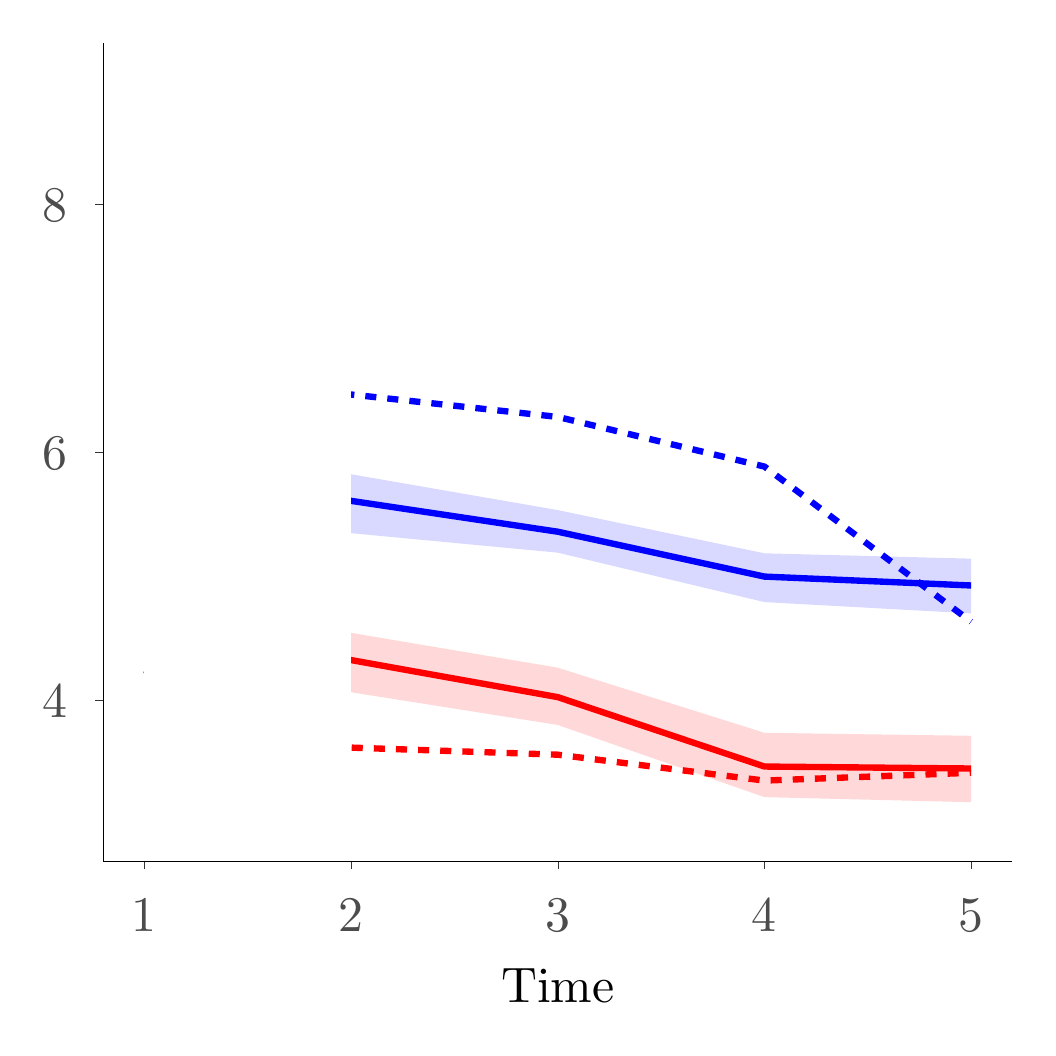
\begin{tikzpicture}[x=1pt,y=1pt]
\definecolor{fillColor}{RGB}{255,255,255}
\path[use as bounding box,fill=fillColor,fill opacity=0.00] (0,0) rectangle (361.35,361.35);
\begin{scope}
\path[clip] (  0.00,  0.00) rectangle (361.35,361.35);
\definecolor{drawColor}{RGB}{255,255,255}
\definecolor{fillColor}{RGB}{255,255,255}

\path[draw=drawColor,line width= 0.1pt,line join=round,line cap=round,fill=fillColor] (  0.00,  0.00) rectangle (361.35,361.35);
\end{scope}
\begin{scope}
\path[clip] ( 27.25, 60.04) rectangle (355.85,355.85);
\definecolor{fillColor}{RGB}{255,255,255}

\path[fill=fillColor] ( 27.25, 60.04) rectangle (355.85,355.85);
\definecolor{fillColor}{RGB}{255,0,0}

\path[fill=fillColor,fill opacity=0.15] ( 42.18,153.97) --
	(116.87,142.66) --
	(191.55,130.08) --
	(266.23,106.55) --
	(340.91,105.47) --
	(340.91, 81.47) --
	(266.23, 83.30) --
	(191.55,109.38) --
	(116.87,121.20) --
	( 42.18,126.81) --
	cycle;

\path[] ( 42.18,153.97) --
	(116.87,142.66) --
	(191.55,130.08) --
	(266.23,106.55) --
	(340.91,105.47);

\path[] (340.91, 81.47) --
	(266.23, 83.30) --
	(191.55,109.38) --
	(116.87,121.20) --
	( 42.18,126.81);
\definecolor{drawColor}{RGB}{255,0,0}

\path[draw=drawColor,line width= 2.3pt,line join=round] ( 42.18,140.95) --
	(116.87,132.83) --
	(191.55,119.44) --
	(266.23, 94.36) --
	(340.91, 93.65);

\path[draw=drawColor,line width= 2.3pt,dash pattern=on 4pt off 4pt ,line join=round] ( 42.18,129.25) --
	(116.87,101.20) --
	(191.55, 98.64) --
	(266.23, 89.28) --
	(340.91, 92.11);
\definecolor{fillColor}{RGB}{0,0,255}

\path[fill=fillColor,fill opacity=0.15] ( 42.18,206.89) --
	(116.87,199.98) --
	(191.55,187.03) --
	(266.23,171.41) --
	(340.91,169.48) --
	(340.91,149.70) --
	(266.23,153.78) --
	(191.55,171.64) --
	(116.87,178.68) --
	( 42.18,175.82) --
	cycle;

\path[] ( 42.18,206.89) --
	(116.87,199.98) --
	(191.55,187.03) --
	(266.23,171.41) --
	(340.91,169.48);

\path[] (340.91,149.70) --
	(266.23,153.78) --
	(191.55,171.64) --
	(116.87,178.68) --
	( 42.18,175.82);
\definecolor{drawColor}{RGB}{0,0,255}

\path[draw=drawColor,line width= 2.3pt,line join=round] ( 42.18,190.35) --
	(116.87,190.36) --
	(191.55,179.21) --
	(266.23,163.00) --
	(340.91,159.78);

\path[draw=drawColor,line width= 2.3pt,dash pattern=on 4pt off 4pt ,line join=round] ( 42.18,233.50) --
	(116.87,228.79) --
	(191.55,220.69) --
	(266.23,202.75) --
	(340.91,146.69);
\definecolor{fillColor}{RGB}{255,255,255}

\path[fill=fillColor] ( 42.18, 60.04) rectangle (116.87,355.85);

\path[fill=fillColor] ( 42.18, 60.04) rectangle (116.87,355.85);

\path[fill=fillColor] ( 42.18, 60.04) rectangle (116.87,355.85);

\path[fill=fillColor] ( 42.18, 60.04) rectangle (116.87,355.85);

\path[fill=fillColor] ( 42.18, 60.04) rectangle (116.87,355.85);
\end{scope}
\begin{scope}
\path[clip] (  0.00,  0.00) rectangle (361.35,361.35);
\definecolor{drawColor}{RGB}{0,0,0}

\path[draw=drawColor,line width= 0.1pt,line join=round] ( 27.25, 60.04) --
	( 27.25,355.85);
\end{scope}
\begin{scope}
\path[clip] (  0.00,  0.00) rectangle (361.35,361.35);
\definecolor{drawColor}{gray}{0.30}

\node[text=drawColor,anchor=base east,inner sep=0pt, outer sep=0pt, scale=  1.80] at ( 14.50,112.11) {4};

\node[text=drawColor,anchor=base east,inner sep=0pt, outer sep=0pt, scale=  1.80] at ( 14.50,201.75) {6};

\node[text=drawColor,anchor=base east,inner sep=0pt, outer sep=0pt, scale=  1.80] at ( 14.50,291.39) {8};
\end{scope}
\begin{scope}
\path[clip] (  0.00,  0.00) rectangle (361.35,361.35);
\definecolor{drawColor}{gray}{0.20}

\path[draw=drawColor,line width= 0.1pt,line join=round] ( 24.50,118.31) --
	( 27.25,118.31);

\path[draw=drawColor,line width= 0.1pt,line join=round] ( 24.50,207.95) --
	( 27.25,207.95);

\path[draw=drawColor,line width= 0.1pt,line join=round] ( 24.50,297.58) --
	( 27.25,297.58);
\end{scope}
\begin{scope}
\path[clip] (  0.00,  0.00) rectangle (361.35,361.35);
\definecolor{drawColor}{RGB}{0,0,0}

\path[draw=drawColor,line width= 0.1pt,line join=round] ( 27.25, 60.04) --
	(355.85, 60.04);
\end{scope}
\begin{scope}
\path[clip] (  0.00,  0.00) rectangle (361.35,361.35);
\definecolor{drawColor}{gray}{0.20}

\path[draw=drawColor,line width= 0.1pt,line join=round] ( 42.18, 57.29) --
	( 42.18, 60.04);

\path[draw=drawColor,line width= 0.1pt,line join=round] (116.87, 57.29) --
	(116.87, 60.04);

\path[draw=drawColor,line width= 0.1pt,line join=round] (191.55, 57.29) --
	(191.55, 60.04);

\path[draw=drawColor,line width= 0.1pt,line join=round] (266.23, 57.29) --
	(266.23, 60.04);

\path[draw=drawColor,line width= 0.1pt,line join=round] (340.91, 57.29) --
	(340.91, 60.04);
\end{scope}
\begin{scope}
\path[clip] (  0.00,  0.00) rectangle (361.35,361.35);
\definecolor{drawColor}{gray}{0.30}

\node[text=drawColor,anchor=base,inner sep=0pt, outer sep=0pt, scale=  1.80] at ( 42.18, 34.90) {1};

\node[text=drawColor,anchor=base,inner sep=0pt, outer sep=0pt, scale=  1.80] at (116.87, 34.90) {2};

\node[text=drawColor,anchor=base,inner sep=0pt, outer sep=0pt, scale=  1.80] at (191.55, 34.90) {3};

\node[text=drawColor,anchor=base,inner sep=0pt, outer sep=0pt, scale=  1.80] at (266.23, 34.90) {4};

\node[text=drawColor,anchor=base,inner sep=0pt, outer sep=0pt, scale=  1.80] at (340.91, 34.90) {5};
\end{scope}
\begin{scope}
\path[clip] (  0.00,  0.00) rectangle (361.35,361.35);
\definecolor{drawColor}{RGB}{0,0,0}

\node[text=drawColor,anchor=base,inner sep=0pt, outer sep=0pt, scale=  1.80] at (191.55,  9.00) {Time};
\end{scope}
\end{tikzpicture}
